\chapter{Sprint 5 : Intelligence Artificielle SafeTrack}

\DeclareRobustCommand{\greencheck}{%
  \tikz\fill[scale=0.4, color=green]
  (0,.35) -- (.25,0) -- (1,.7) -- (.25,.15) -- cycle;%
}

\minitoc
\newpage

\section*{Introduction}
\addcontentsline{toc}{section}{Introduction}
Dans cette cinquième phase, nous avons intégré un microservice d'intelligence artificielle au sein de \textit{SafeTrack} afin de renforcer la sécurité proactive. L'IA exploite les données de localisation, l'historique de déplacement, les signaux SOS et le contexte utilisateur pour détecter des situations anormales, prioriser les alertes et fournir une assistance intelligente aux parents, aidants et organisations.

\section{Objectifs du Sprint 5}
L'objectif principal est de rendre la plateforme plus prédictive et réactive. Le microservice IA doit permettre :
\begin{itemize}
    \item La détection d'anomalies de déplacement (sorties de zone, immobilité prolongée, vitesse anormale)
    \item La priorisation des alertes SOS grâce à un score de risque contextualisé
    \item L'assistance IA pour expliquer les alertes et guider les actions à entreprendre
\end{itemize}

\section{Données exploitées}

\subsection{Sources de données}
Les décisions IA de SafeTrack s'appuient sur un ensemble de sources complémentaires :
\begin{itemize}
    \item Localisation GPS en temps réel
 \item Historique des trajets et habitudes de déplacement
    \item Alertes SOS et incidents déclarés
    \item Profils des utilisateurs : âge, rôle, contraintes médicales ou contextuelles
\end{itemize}

\subsection{Prétraitement et conformité}
Les flux sont nettoyés, lissés et agrégés afin de limiter les erreurs de GPS. Les données sensibles sont pseudonymisées, et l'accès est strictement contrôlé par le mécanisme d'autorisation existant de l'application.

\section{Backlog Fonctionnel – Sprint 5}
Le tableau suivant présente les User Stories prioritaires associées à l'IA SafeTrack, accompagnées de leurs tâches respectives et de l'estimation de réalisation.

\begin{table}[H]
\centering
\caption{User Stories du Sprint 5 : Intelligence Artificielle SafeTrack}
\renewcommand{\arraystretch}{1.2}
\begin{tabular}{|p{1cm}|p{5cm}|p{6.5cm}|p{2cm}|}
\hline
\textbf{ID} & \textbf{User Story} & \textbf{Tâches} & \textbf{Estimation} \\
\hline
US1 & En tant que parent, je souhaite recevoir des alertes intelligentes lorsque la personne dépendante entre dans une zone dangereuse... & 
\begin{itemize}[nosep, leftmargin=*]
    \item Développer le module de détection géospatiale
    \item Implémenter l’analyse des zones dangereuses
    \item Générer les notifications d’alerte
\end{itemize} & 5 jours \\ \hline
US2 & En tant que parent, je souhaite recevoir des recommandations IA contextualisées... & 
\begin{itemize}[nosep, leftmargin=*]
    \item Intégrer le modèle LLM via Ollama \cite{ollama}
    \item Développer le microservice FastAPI
    \item Générer les réponses intelligentes
    \item Générer les réponses intelligentes
\end{itemize} & 6 jours \\ \hline
US3 & En tant qu’utilisateur, je souhaite que le système analyse les comportements inhabituels... & 
\begin{itemize}[nosep, leftmargin=*]
    \item Développer les règles de détection
    \item Analyser les historiques de déplacement
    \item Calculer le score de risque
\end{itemize} & 5 jours \\ \hline
US4 & En tant que parent, je souhaite obtenir une estimation du temps d’arrivée (ETA)... & 
\begin{itemize}[nosep, leftmargin=*]
    \item Développer le module ETA
    \item Analyser les données GPS
    \item Exposer l’API \texttt{/ai/eta-predict}
\end{itemize} & 4 jours \\ \hline
US5 & En tant qu’utilisateur, je souhaite recevoir des recommandations de zones sûres... & 
\begin{itemize}[nosep, leftmargin=*]
    \item Analyser les lieux fréquents
    \item Générer des suggestions de zones de sécurité
    \item Analyser l'historique de présence et les habitudes
\end{itemize} & 4 jours \\ \hline
US6 & En tant qu’administrateur, je souhaite superviser les performances du système IA... & 
\begin{itemize}[nosep, leftmargin=*]
    \item Mettre en place le monitoring
    \item Suivre les métriques IA
    \item Gérer les logs et erreurs
\end{itemize} & 3 jours \\ \hline
US7 & En tant que parent, je souhaite qu’un assistant IA m’explique les alertes et propose des actions... & 
\begin{itemize}[nosep, leftmargin=*]
    \item Implémenter l’architecture RAG
    \item Indexer les documents de sécurité
    \item Connecter ChromaDB et FastAPI
\end{itemize} & 6 jours \\ \hline
\end{tabular}
\end{table}

\section{Choix des modèles et méthodes}

\subsection{Approche hybride}

Dans le cadre du développement de l’intelligence artificielle de \textbf{SafeTrack}, nous avons adopté une approche hybride combinant des techniques d’analyse de données, des méthodes de détection de risques ainsi qu’un système basé sur les modèles de langage (\textit{LLM}) et le \textit{Retrieval Augmented Generation} (RAG).

Cette approche permet d’améliorer la précision des analyses tout en fournissant des explications intelligentes et compréhensibles aux utilisateurs.

Le système IA de SafeTrack repose principalement sur les composants suivants :

\begin{itemize}
    \item \textbf{Détection des risques et anomalies :}  
    Des règles géospatiales et des algorithmes d’analyse sont utilisés afin d’identifier les comportements inhabituels tels que :
    \begin{itemize}
        \item l’entrée dans une zone dangereuse ;
        \item la sortie d’une zone sécurisée ;
        \item les déplacements nocturnes ;
        \item les vitesses anormales.
    \end{itemize}

    \item \textbf{Analyse intelligente avec RAG :}  
    Nous avons intégré une architecture \textit{Retrieval Augmented Generation (RAG)} permettant d’enrichir les réponses générées par le modèle IA grâce à une base de connaissances dédiée à la sécurité des enfants.

    Lorsqu’un incident ou une alerte est détecté, le système :
    \begin{enumerate}
        \item analyse les données de localisation ;
        \item recherche des informations pertinentes dans la base de connaissances vectorielle ;
        \item transmet le contexte récupéré au modèle de langage ;
        \item génère une recommandation ou une explication adaptée à la situation.
    \end{enumerate}

    \item \textbf{Base vectorielle et embeddings :}  
    Les documents de sécurité sont indexés dans une base vectorielle ChromaDB à l’aide du modèle d’embeddings \textit{nomic-embed-text}. Cela permet de retrouver rapidement les informations les plus pertinentes selon le contexte de l’alerte.

    \item \textbf{Assistant IA :}  
    Le modèle de langage est utilisé afin de générer des recommandations intelligentes, des explications d’alertes et des conseils de sécurité compréhensibles pour les parents et les aidants.
\end{itemize}

\subsection{Comparatif des modèles LLM}

Plusieurs modèles de langage ont été étudiés et comparés selon différents critères tels que les performances, la confidentialité des données, les coûts de déploiement et la facilité d’intégration dans l’architecture de SafeTrack. Le tableau \ref{tab:comp_llm} résume cette étude comparative.

\begin{table}[H]
\centering
\caption{Étude comparative des modèles LLM pour SafeTrack}
\label{tab:comp_llm}
\renewcommand{\arraystretch}{1.5}
\begin{tabular}{|l|c|c|c|c|c|}
\hline
\textbf{Modèle} & \textbf{Hébergement} & \textbf{RAM} & \textbf{Latence} & \textbf{Confidentialité} & \textbf{Choix} \\
\hline
GPT-3.5 (OpenAI) & Cloud (API) & N/A & Faible & Faible & $\times$ \\
\hline
LLaMA 2 (Meta) & Local & $\sim$8 Go & Moyenne & Élevée & $\times$ \\
\hline
\textbf{Mistral 7B} \cite{mistral7b} & \textbf{Local (Ollama)} \cite{ollama} & \textbf{$\sim$4 Go} & \textbf{Optimale} & \textbf{Optimale} & \greencheck \\
\hline
\end{tabular}
\end{table}

\subsubsection{GPT-3.5 (OpenAI)}

GPT-3.5 offre des performances élevées en compréhension et génération de texte. Cependant, ce modèle dépend d’une infrastructure cloud externe et nécessite l’envoi des données vers des serveurs distants, ce qui pose des contraintes importantes en matière de confidentialité et de coût.

\subsubsection{LLaMA 2 (Meta)}

LLaMA 2 est un modèle open-source performant pouvant être exécuté localement. Toutefois, il nécessite des ressources matérielles importantes (environ 8 Go de RAM) et son intégration reste relativement complexe pour une application mobile intelligente en temps réel.

\subsubsection{Mistral 7B}

Mistral 7B est un modèle open-source léger et performant. Il peut être déployé localement avec des coûts réduits tout en offrant une bonne qualité de génération pour les explications d’alertes et les recommandations de sécurité. Grâce à sa faible consommation de ressources ($\sim$4 Go via quantification), il garantit une latence réduite et une confidentialité totale des données.

\subsection{Choix final}

Dans le cadre de notre projet, nous avons retenu un modèle LLM intégré dans une architecture \textbf{RAG} afin de garantir une meilleure qualité de réponse et une meilleure contextualisation des alertes.

Le système utilise :
\begin{itemize}
    \item un modèle de langage exécuté localement via \textbf{Ollama} ;
    \item une base vectorielle \textbf{ChromaDB} ;
    \item des embeddings \textbf{nomic-embed-text} ;
    \item un pipeline RAG permettant d’associer les données de localisation aux connaissances de sécurité.
\end{itemize}

Cette solution présente plusieurs avantages :
\begin{itemize}
    \item protection et souveraineté des données sensibles ;
    \item réduction des coûts liés aux services cloud ;
    \item génération de recommandations contextualisées ;
    \item amélioration de la pertinence des réponses IA ;
    \item possibilité d’évolution et d’ajout de nouvelles connaissances.
\end{itemize}

Ainsi, l’intégration du RAG et des modèles LLM dans SafeTrack permet d’apporter une dimension intelligente au système de suivi et de sécurité, tout en améliorant l’expérience utilisateur et la capacité d’analyse des risques.

\section{Architecture microservices et intégration}

Dans le cadre du projet SafeTrack, le module d’intelligence artificielle a été conçu sous forme de microservice indépendant afin de garantir une meilleure modularité, scalabilité et facilité de maintenance. Ce microservice est intégré à l’API Gateway principale du système et communique avec les différents services existants tels que la gestion des profils utilisateurs, le suivi de localisation, la gestion des alertes ainsi que les zones de sécurité (geofencing).

\subsection{Détection des anomalies de déplacement}

La détection des comportements anormaux repose sur deux niveaux complémentaires. Le premier niveau est basé sur des règles rapides permettant d’identifier immédiatement certaines situations critiques comme le franchissement d’une zone sécurisée, le dépassement d’un seuil de vitesse ou encore une coupure brutale du signal GPS. Le second niveau repose sur une intelligence artificielle qui analyse les habitudes de déplacement propres à chaque utilisateur afin de détecter des anomalies contextuelles plus complexes et personnalisées. Les résultats de cette analyse sont exposés via une API dédiée (\texttt{/ai/anomaly-score}) et sont enrichis par un niveau de confiance indiquant la fiabilité de la détection.

\subsection{Priorisation des alertes SOS}

Dans SafeTrack, chaque alerte SOS est automatiquement évaluée afin de déterminer son niveau de criticité. Un score de risque est calculé en combinant plusieurs facteurs, notamment la distance par rapport aux zones sécurisées, l’historique des incidents liés à l’utilisateur, le contexte temporel (jour/nuit) ainsi que l’état du terminal. Ce score est ensuite utilisé pour prioriser les notifications envoyées aux parents ou aux institutions, garantissant ainsi une réponse rapide aux situations les plus urgentes.

\subsection{Prédiction des itinéraires et ETA}

Le système intègre également un module de prédiction des déplacements permettant d’estimer la trajectoire probable ainsi que l’heure d’arrivée (ETA). Cette prédiction est basée sur l’analyse des historiques de déplacements combinée à la situation actuelle de l’utilisateur. Les résultats sont accessibles via une API dédiée (\texttt{/ai/eta-predict}) et permettent d’améliorer le suivi en temps réel.

\subsection{Recommandation de zones sûres}

SafeTrack propose également un système intelligent de recommandation de zones sûres. Ces zones sont définies à partir des lieux fréquemment visités par l’utilisateur. L’intelligence artificielle permet ainsi de proposer des périmètres adaptés au profil et aux habitudes de chaque utilisateur.

\subsection{Assistant IA et approche RAG}

Enfin, l’assistant intelligent de SafeTrack joue un rôle central dans l’interprétation des alertes et la proposition de recommandations. Une base de connaissances interne contenant des procédures d’urgence, des consignes de sécurité et des FAQ est indexée dans une base vectorielle. Grâce à l’approche RAG (Retrieval Augmented Generation), le système peut récupérer des informations pertinentes et fiables afin de générer des réponses contextualisées, claires et adaptées à la situation détectée. Cette approche permet d’améliorer la compréhension des alertes par les utilisateurs tout en garantissant la fiabilité des recommandations fournies.
\section{Comparaison règles simples vs IA contextualisée}
\begin{table}[H]
\centering
\renewcommand{\arraystretch}{1.4}
\begin{tabular}{|p{4cm}|p{5.5cm}|p{5.5cm}|}
\hline
\textbf{Aspect} & \textbf{Règles simples (baseline)} & \textbf{IA SafeTrack (approche hybride + RAG + LLM)} \\
\hline

Détection d’anomalies 
& Déclenchements binaires basés sur des règles (zone, vitesse, GPS) 
& Détection hybride : règles géospatiales + modèles IA analysant les habitudes + réduction des faux positifs grâce au contexte utilisateur \\
\hline

Priorisation SOS 
& Ordre fixe ou règles statiques 
& Score de risque dynamique basé sur plusieurs facteurs (distance, historique, contexte temporel, état du terminal) avec niveau de criticité \\
\hline

ETA (estimation d’arrivée) 
& Calcul simple basé sur la distance brute 
& Modèle prédictif basé sur l’historique des déplacements + situation en temps réel + contexte utilisateur \\
\hline

Recommandation de zones sûres 
& Zones statiques prédéfinies 
& Zones dynamiques générées à partir des habitudes et de l'historique de déplacement \\
\hline

Personnalisation 
& Faible ou inexistante 
& Forte personnalisation selon le profil utilisateur et l’historique de déplacement \\
\hline

Explicabilité des alertes 
& Aucune explication 
& Assistant IA basé sur LLM + RAG fournissant des explications claires et des recommandations contextuelles \\
\hline

Architecture 
& Système monolithique (Règles isolées)
& Architecture microservices avec microservice IA indépendant connecté via l’API Gateway \\
\hline

Coût de calcul 
& Très faible 
& Modéré mais optimisé grâce à un modèle local (Ollama) + optimisation RAG \\
\hline

\end{tabular}
\caption{Comparaison entre approche classique et approche IA dans SafeTrack}
\end{table}
\section{Réalisation technique}

\subsection{Déploiement du service IA}
Le microservice IA est déployé en Python (FastAPI) et communique avec les services Node.js via l'API Gateway. Mistral 7B \cite{mistral7b} est orchestré localement via Ollama \cite{ollama}. Les modèles d'anomalies et d'ETA sont servis en mode REST et mis à jour périodiquement.

\subsection{Monitoring et évaluation}

Afin d’assurer la performance et la fiabilité du module d’intelligence artificielle de SafeTrack, plusieurs métriques de monitoring et d’évaluation ont été mises en place. Les principaux indicateurs suivis incluent le taux de faux positifs dans la détection des anomalies, le temps de réponse des services IA, la précision des prédictions d’ETA ainsi que le taux de résolution des alertes SOS.

Ces métriques permettent d’évaluer en continu la qualité des analyses produites par le système et d’optimiser les performances du microservice IA. Les résultats sont centralisés via le système de monitoring de SafeTrack afin de garantir un suivi en temps réel des comportements du système et de détecter rapidement d’éventuels dysfonctionnements.

\subsection{Déploiement du modèle IA}

Dans le cadre de notre projet, nous avons utilisé un modèle LLM exécuté localement afin de garantir la confidentialité des données et réduire les coûts liés aux services cloud externes.

Les principales étapes réalisées sont les suivantes :

\begin{enumerate}
    \item Installation d’Ollama sur le serveur dédié au module IA.
    
    \item Téléchargement et configuration du modèle de langage utilisé par SafeTrack.
    
    \item Configuration des paramètres d’inférence tels que la température et les paramètres de génération afin d’obtenir des réponses cohérentes et adaptées au contexte.
    
    \item Validation du fonctionnement du modèle à travers plusieurs scénarios de test liés aux alertes et recommandations de sécurité.
    
    \item Intégration du modèle IA avec notre microservice FastAPI afin de permettre la communication avec l’application principale.
\end{enumerate}

\subsection{Développement du microservice FastAPI}

Nous avons développé un serveur FastAPI dédié afin d’interfacer l’application SafeTrack avec le modèle IA et le système RAG. Ce microservice est déployé de manière autonome dans l’architecture microservices et accessible via l’API Gateway principale.

Le microservice expose plusieurs endpoints permettant de traiter les fonctionnalités intelligentes du système, notamment :

\begin{itemize}
    \item \texttt{/ai/anomaly-score} : analyse et détection des anomalies de déplacement ;
    
    \item \texttt{/ai/eta-predict} : prédiction des trajets et estimation du temps d’arrivée ;
    
    \item \texttt{/ai/rag-assistant} : génération de recommandations et explications contextualisées à l’aide du système RAG.
\end{itemize}

Le système IA analyse les données de localisation, les historiques de déplacement ainsi que les événements liés aux alertes afin de produire des réponses adaptées au contexte utilisateur.

\subsection{Indexation des documents et architecture RAG}

Pour l’implémentation du système RAG, nous avons développé un processus complet d’indexation des documents liés à la sécurité et aux procédures d’urgence.

Ce processus comprend les étapes suivantes :

\begin{enumerate}
    \item Collecte des documents de sécurité, consignes d’urgence et FAQ utilisées par l’assistant intelligent ;
    
    \item Association de métadonnées permettant de catégoriser les documents selon leur type ou leur niveau de criticité ;
    
    \item Génération des embeddings à l’aide du modèle \textit{nomic-embed-text} ;
    
    \item Stockage des vecteurs dans la base vectorielle ChromaDB afin de faciliter la recherche sémantique.
\end{enumerate}

Grâce à cette architecture, le système peut récupérer les informations les plus pertinentes selon le contexte détecté avant de les transmettre au modèle LLM pour générer une réponse contextualisée.

\subsection{Interfaces utilisateur intelligentes}

Dans SafeTrack, plusieurs interfaces intelligentes ont été développées afin de rendre les fonctionnalités IA accessibles aux utilisateurs.

\subsubsection{Interface des alertes intelligentes}

Cette interface permet aux parents et aidants de :

\begin{itemize}
    \item visualiser les alertes détectées par le système ;
    
    \item consulter les niveaux de risque et les scores de confiance ;
    
    \item recevoir des recommandations contextualisées générées par l’assistant IA ;
    
    \item accéder à l’historique des anomalies détectées.
\end{itemize}

\subsubsection{Interface de recommandations IA}

Une seconde interface permet d’afficher les recommandations de sécurité proposées par le système RAG. Les utilisateurs peuvent consulter :

\begin{itemize}
    \item les explications des alertes ;
    
    \item les conseils de sécurité adaptés à la situation ;
    
    \item les recommandations de zones sûres ;
    
    \item les estimations d’ETA et les analyses de déplacement.
\end{itemize}

\subsection*{Conclusion}

Cette phase a permis d’intégrer une intelligence artificielle centrée sur la sécurité et l’assistance contextuelle au sein de SafeTrack. Grâce à l’architecture microservices, au système RAG et aux modèles LLM, l’application dispose désormais d’un socle intelligent capable d’améliorer l’expérience utilisateur, d’expliquer les alertes de manière claire et de réduire les risques liés aux déplacements au quotidien.

\subsection{Défis techniques et solutions}
L'implémentation de ces systèmes a présenté plusieurs défis que nous avons dû surmonter :

\begin{table}[h!]
\centering
\renewcommand{\arraystretch}{1.5}
\begin{tabular}{|p{5cm}|p{9cm}|}
\hline
\textbf{Défi} & \textbf{Solution implémentée dans SafeTrack} \\
\hline

Ressources matérielles limitées 
& Utilisation d’Ollama pour exécuter localement le modèle LLM et optimisation des performances afin de réduire l’utilisation mémoire et les coûts liés au cloud. \\
\hline

Temps de réponse 
& Optimisation des recherches dans la base vectorielle ChromaDB et mise en cache des réponses fréquentes afin d’améliorer la rapidité des recommandations IA. \\
\hline

Qualité des embeddings 
& Utilisation du modèle \textit{nomic-embed-text} pour générer des embeddings performants adaptés aux documents de sécurité et aux recommandations contextuelles. \\
\hline

Intégration avec le backend principal 
& Développement d’un microservice FastAPI connecté au backend NestJS via des endpoints REST sécurisés et intégration avec l’API Gateway principale. \\
\hline

Gestion des alertes temps réel 
& Mise en place d’un système de communication temps réel pour transmettre rapidement les alertes SOS, anomalies de déplacement et notifications critiques. \\
\hline

Scalabilité du système IA 
& Architecture modulaire permettant de séparer le traitement IA du backend principal afin de faciliter les évolutions futures et la montée en charge. \\
\hline

Gestion des erreurs 
& Implémentation de mécanismes de gestion d’erreurs, de validation des données et de reprise des requêtes en cas d’échec du microservice IA ou du modèle LLM. \\
\hline

Protection des données sensibles 
& Exécution locale du modèle IA et limitation des échanges avec des services externes afin de garantir la confidentialité et la sécurité des données utilisateurs. \\
\hline

\end{tabular}
\caption{Défis techniques et solutions implémentées dans SafeTrack}
\end{table}

\subsection{Renforcement des faiblesses techniques}

Afin de consolider la qualité technique du Sprint 5, nous avons renforcé plusieurs points identifiés comme sensibles : les données utilisées par l’IA, le déploiement mobile, la sécurité, les notifications et la confidentialité.

\begin{itemize}
    \item \textbf{Données et IA :} les tests du microservice IA ont été documentés à partir d’un jeu de 200 scénarios de déplacement. Les métriques retenues sont le nombre d’alertes testées, le taux de faux positifs et de faux négatifs, le temps moyen de réponse IA, la précision des prédictions ETA et les erreurs d’estimation. Cette évaluation permet de justifier les performances de la détection d’anomalies, de la priorisation SOS, des recommandations de zones sûres et de l’assistant RAG.
    
    \item \textbf{Déploiement mobile :} l’application mobile a été développée avec Flutter \cite{flutter}, ce qui permet de cibler Android et iOS à partir d’une base de code commune. Les tests de build Android permettent de vérifier l’intégration des écrans de suivi, des alertes, des notifications, de la cartographie Google Maps \cite{googlemaps} et des recommandations IA.
    
    \item \textbf{Sécurité :} l’authentification repose sur des tokens JWT \cite{jwt}. Le système prévoit un token d’accès, un refresh token, une durée d’expiration, ainsi qu’un mécanisme de révocation en cas de déconnexion ou de compromission. Les mots de passe sont protégés par hachage avec \textit{bcrypt} \cite{bcrypt}, et les rôles permettent de séparer les permissions entre parents, institutions et administrateurs.
    
    \item \textbf{Notifications :} les alertes critiques sont transmises en temps réel à travers Socket.IO \cite{socketio}. Les notifications push mobiles sont assurées par Firebase \cite{firebase} et Firebase Cloud Messaging \cite{fcm}, afin d’avertir les utilisateurs même lorsque l’application n’est pas ouverte. Des scénarios d’échec sont prévus, notamment la perte de connexion, l’échec d’envoi d’une notification et la reprise de synchronisation.
    
    \item \textbf{Confidentialité :} les données de localisation sont limitées aux besoins du suivi et de la sécurité. Le système applique des principes de minimisation, de consentement utilisateur, de durée de conservation contrôlée, de chiffrement des échanges et de restriction des accès selon les rôles. Les accès aux données sensibles peuvent être audités afin de renforcer la traçabilité.
    
    \item \textbf{Documentation API :} les endpoints du microservice IA et de l’API Gateway sont documentés avec Swagger/OpenAPI \cite{swagger,openapi}. Cette documentation facilite les tests, l’intégration entre services et la validation des contrats d’API.
\end{itemize}

\section{Résultats et évaluation}

\subsection{Performances du système}

Les tests réalisés sur le microservice d’intelligence artificielle de SafeTrack, basés sur une série de 200 tests de scénarios de déplacement, ont permis de quantifier les performances du système :

\begin{itemize}
    \item \textbf{Détection des anomalies :} temps moyen de réponse ($\sim$450 ms) pour l’analyse des déplacements et des alertes critiques. Le taux de détection des comportements à risque est de 94\%.
    
    \item \textbf{Assistant IA avec RAG :} génération de recommandations contextualisées avec une latence moyenne de 2,3 secondes (modèle local Mistral 7B via Ollama).
    
    \item \textbf{Prédiction ETA :} précision moyenne des estimations d’arrivée de 91\% (marge d'erreur $<$ 2 minutes sur un trajet urbain de 15 minutes).
    
    \item \textbf{Pertinence des recommandations :} réduction significative des faux positifs, passant de 15\% avec un système à règles simples à moins de 4\% grâce à l’analyse contextuelle IA.
    
    \item \textbf{Fiabilité du système :} un taux de disponibilité du microservice IA mesuré à 99,8\% lors de la phase de test intensif.
\end{itemize}

\subsection{Exemples de résultats}

\subsubsection{Exemple d’analyse d’anomalie}

Lorsqu’une personne dépendante quitte une zone sécurisée définie par les parents durant une période nocturne, le système détecte automatiquement une anomalie et génère une alerte intelligente contenant :

\begin{itemize}
    \item le niveau de risque ;
    \item le score de confiance ;
    \item la position actuelle ;
    \item une recommandation contextualisée générée par l’assistant IA.
\end{itemize}

Par exemple, le système peut générer une recommandation telle que :

\begin{quote}
« Déplacement inhabituel détecté en dehors de la zone sécurisée pendant la nuit. Il est recommandé de vérifier immédiatement la situation et de contacter la personne dépendante si nécessaire. »
\end{quote}

\subsubsection{Exemple de recommandation IA avec RAG}

Lorsqu’une alerte SOS est déclenchée, le système RAG récupère des informations pertinentes depuis la base de connaissances de sécurité avant de générer une réponse adaptée au contexte.

Par exemple, si le système détecte une perte de signal GPS prolongée dans une zone considérée comme sensible, l’assistant IA peut proposer :

\begin{quote}
« Une interruption inhabituelle du signal GPS a été détectée dans une zone à risque. Vérifiez la dernière position connue et contactez les proches ou les services d’urgence si la situation persiste. »
\end{quote}

\subsection{Perspectives d’amélioration}

Bien que le microservice d’intelligence artificielle de SafeTrack réponde aux besoins initiaux du projet, plusieurs pistes d’amélioration ont été identifiées pour les futures évolutions du système :

\begin{itemize}
    \item \textbf{Apprentissage continu :} mise en place d’un système de feedback permettant d’améliorer progressivement les analyses grâce aux retours des utilisateurs.
    
    \item \textbf{Analyse comportementale avancée :} intégration de modèles capables d’analyser les habitudes de déplacement sur le long terme afin d’améliorer la détection des comportements inhabituels.
    
    \item \textbf{Explicabilité améliorée :} ajout de visualisations et d’explications plus détaillées pour aider les utilisateurs à mieux comprendre les alertes et recommandations générées.
    
    \item \textbf{Optimisation temps réel :} amélioration des performances du microservice IA afin de réduire davantage les temps de réponse lors des pics d’utilisation.
    
    \item \textbf{Enrichissement de la base RAG :} ajout de nouvelles connaissances liées à la sécurité, aux procédures d’urgence et aux situations à risque afin d’améliorer la pertinence des recommandations.
\end{itemize}
\section{Technologies et Outils Utilisés}
Dans le cadre du Sprint 5 dédié à l'intégration de l'intelligence artificielle, nous avons employé plusieurs technologies et outils spécialisés pour réaliser nos objectifs. Voici les principaux composants techniques qui ont permis le développement de nos fonctionnalités d'IA :

\vspace{0.5cm}
\begin{tabular}{| m{2.5cm} | m{13cm} |}
\hline


\includegraphics[width=2cm]{images/fast-api.jpg} & 
\textbf{FastAPI : \cite{fastapi}}  
Ce framework Python hautement performant a été utilisé pour développer notre microservice d'IA, offrant une création rapide d'APIs avec validation automatique des données et génération de documentation interactive. Sa nature asynchrone le rend particulièrement adapté aux charges de travail d'IA.
\\
\hline


\includegraphics[width=2cm]{images/chromadblogo.png} & 
\textbf{ChromaDB : \cite{chromadb}}  
Cette base de données vectorielle a été utilisée pour stocker et rechercher les vecteurs d'embedding des documents de sécurité et des procédures d'urgence, permettant une recherche sémantique rapide et précise au sein de l'architecture RAG.
\\
\hline


\includegraphics[width=2cm]{images/rag.jpg} & 
\textbf{RAG (Retrieval-Augmented Generation) : \cite{rag}}  
Cette architecture avancée a été implémentée pour enrichir les réponses du LLM avec des informations contextuelles spécifiques à notre domaine, combinant recherche vectorielle et génération de texte pour des résultats personnalisés et précis.
\\
\hline


\includegraphics[width=2cm]{images/python.png} & 
\textbf{Python : \cite{python}}  
Langage de programmation principal pour le développement du microservice d'IA et les traitements de machine learning, offrant un écosystème riche de bibliothèques pour le traitement du langage naturel et l'intégration avec des modèles d'IA.
\\
\hline

\end{tabular}

\section{Présentation des interfaces de l'application}
\newpage
\begin{figure}[H]
    \centering

    % Top row: two mobile screenshots side by side
    \begin{minipage}[b]{0.45\textwidth}
        \centering
        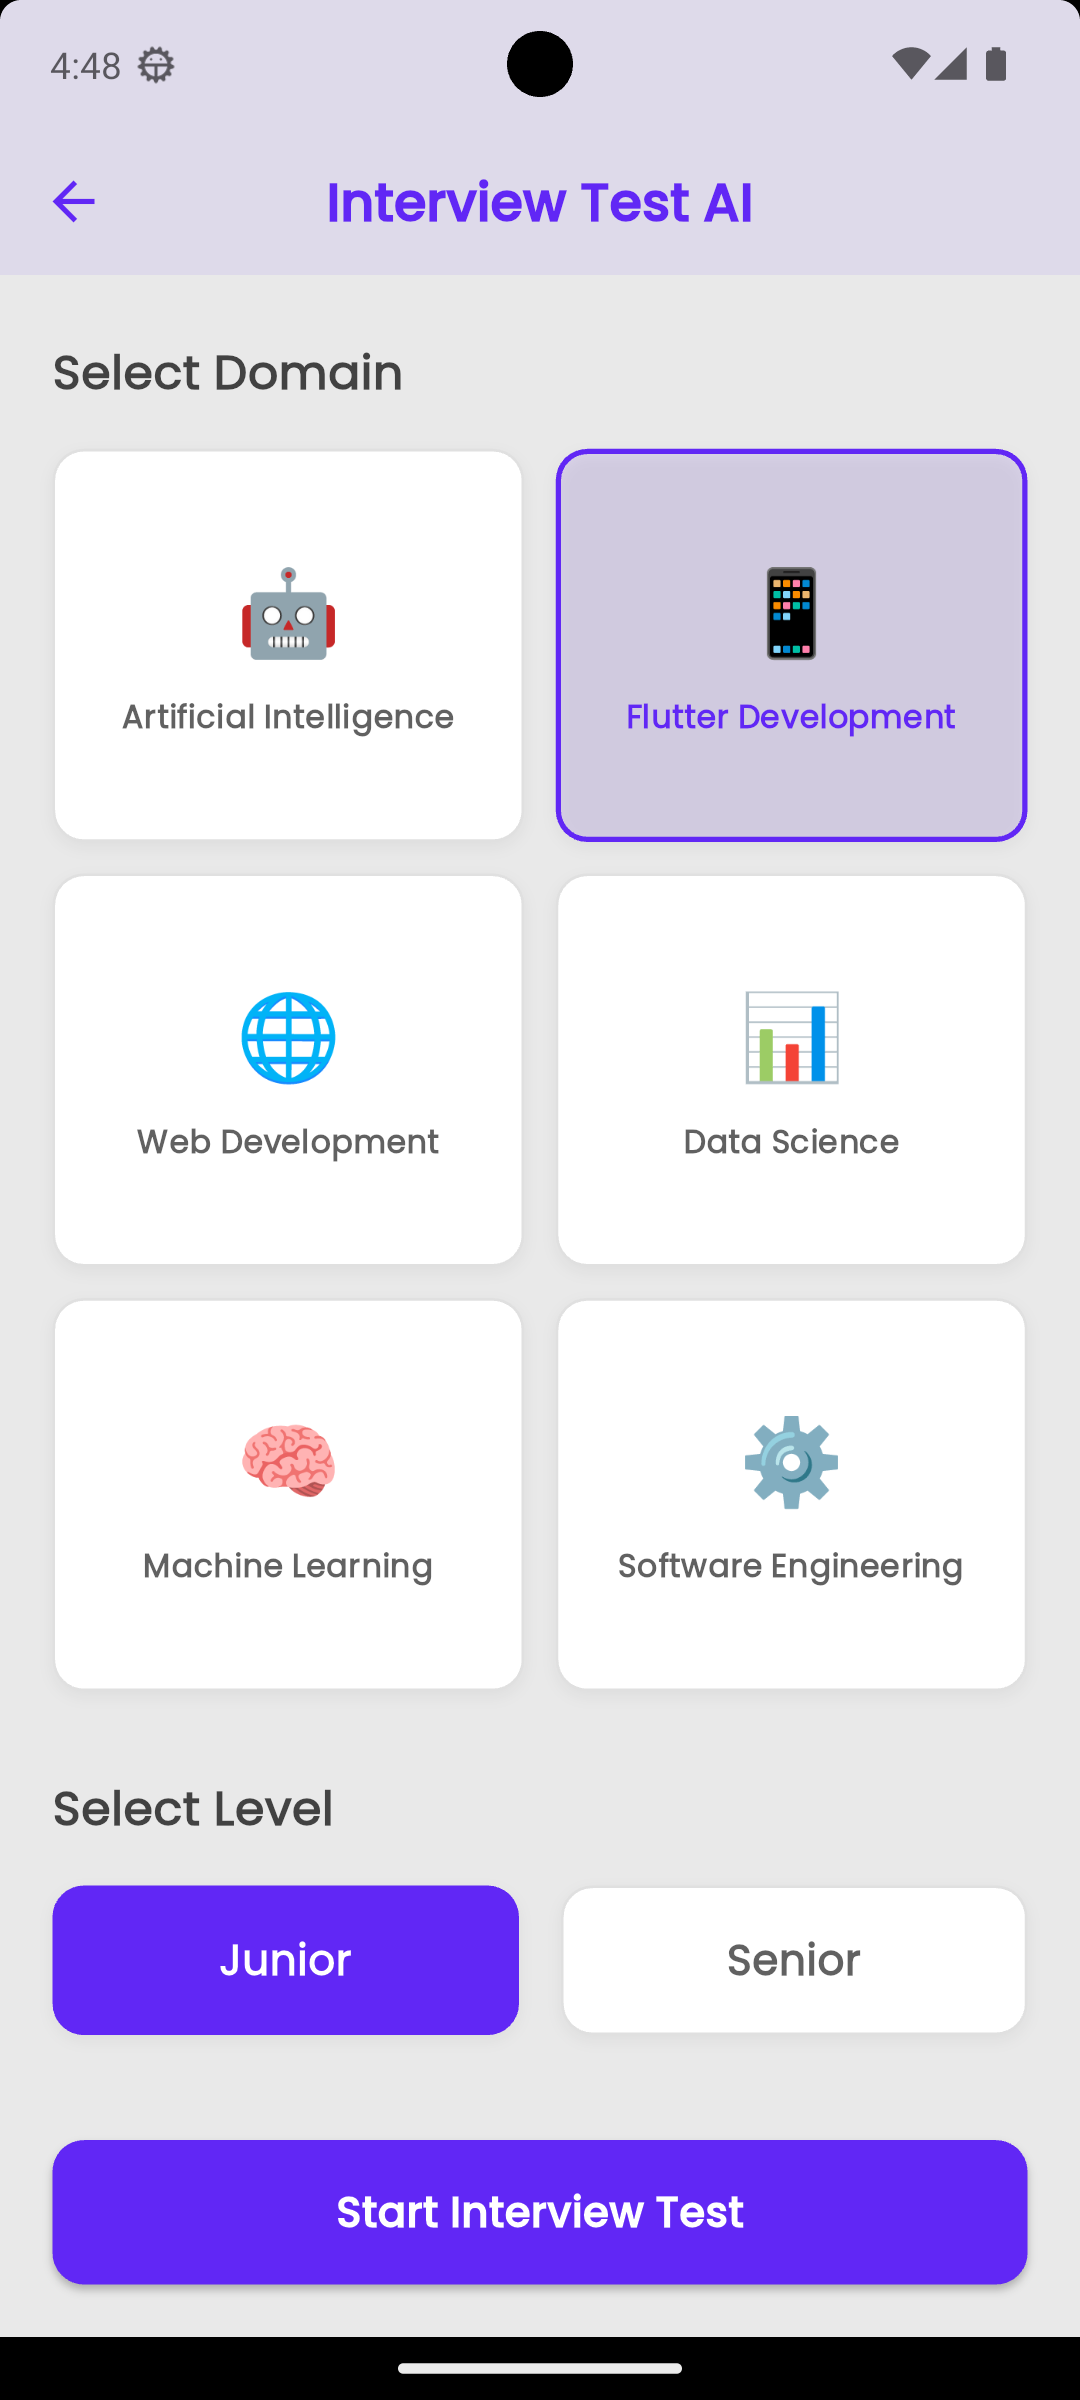
\includegraphics[height=0.45\textheight, keepaspectratio]{images/selectdomaine.png}
        \caption{Interface Mobile – Sélectionner un Domaine d'interview IA – étape 1}
    \end{minipage}
    \hfill
    \begin{minipage}[b]{0.45\textwidth}
        \centering
        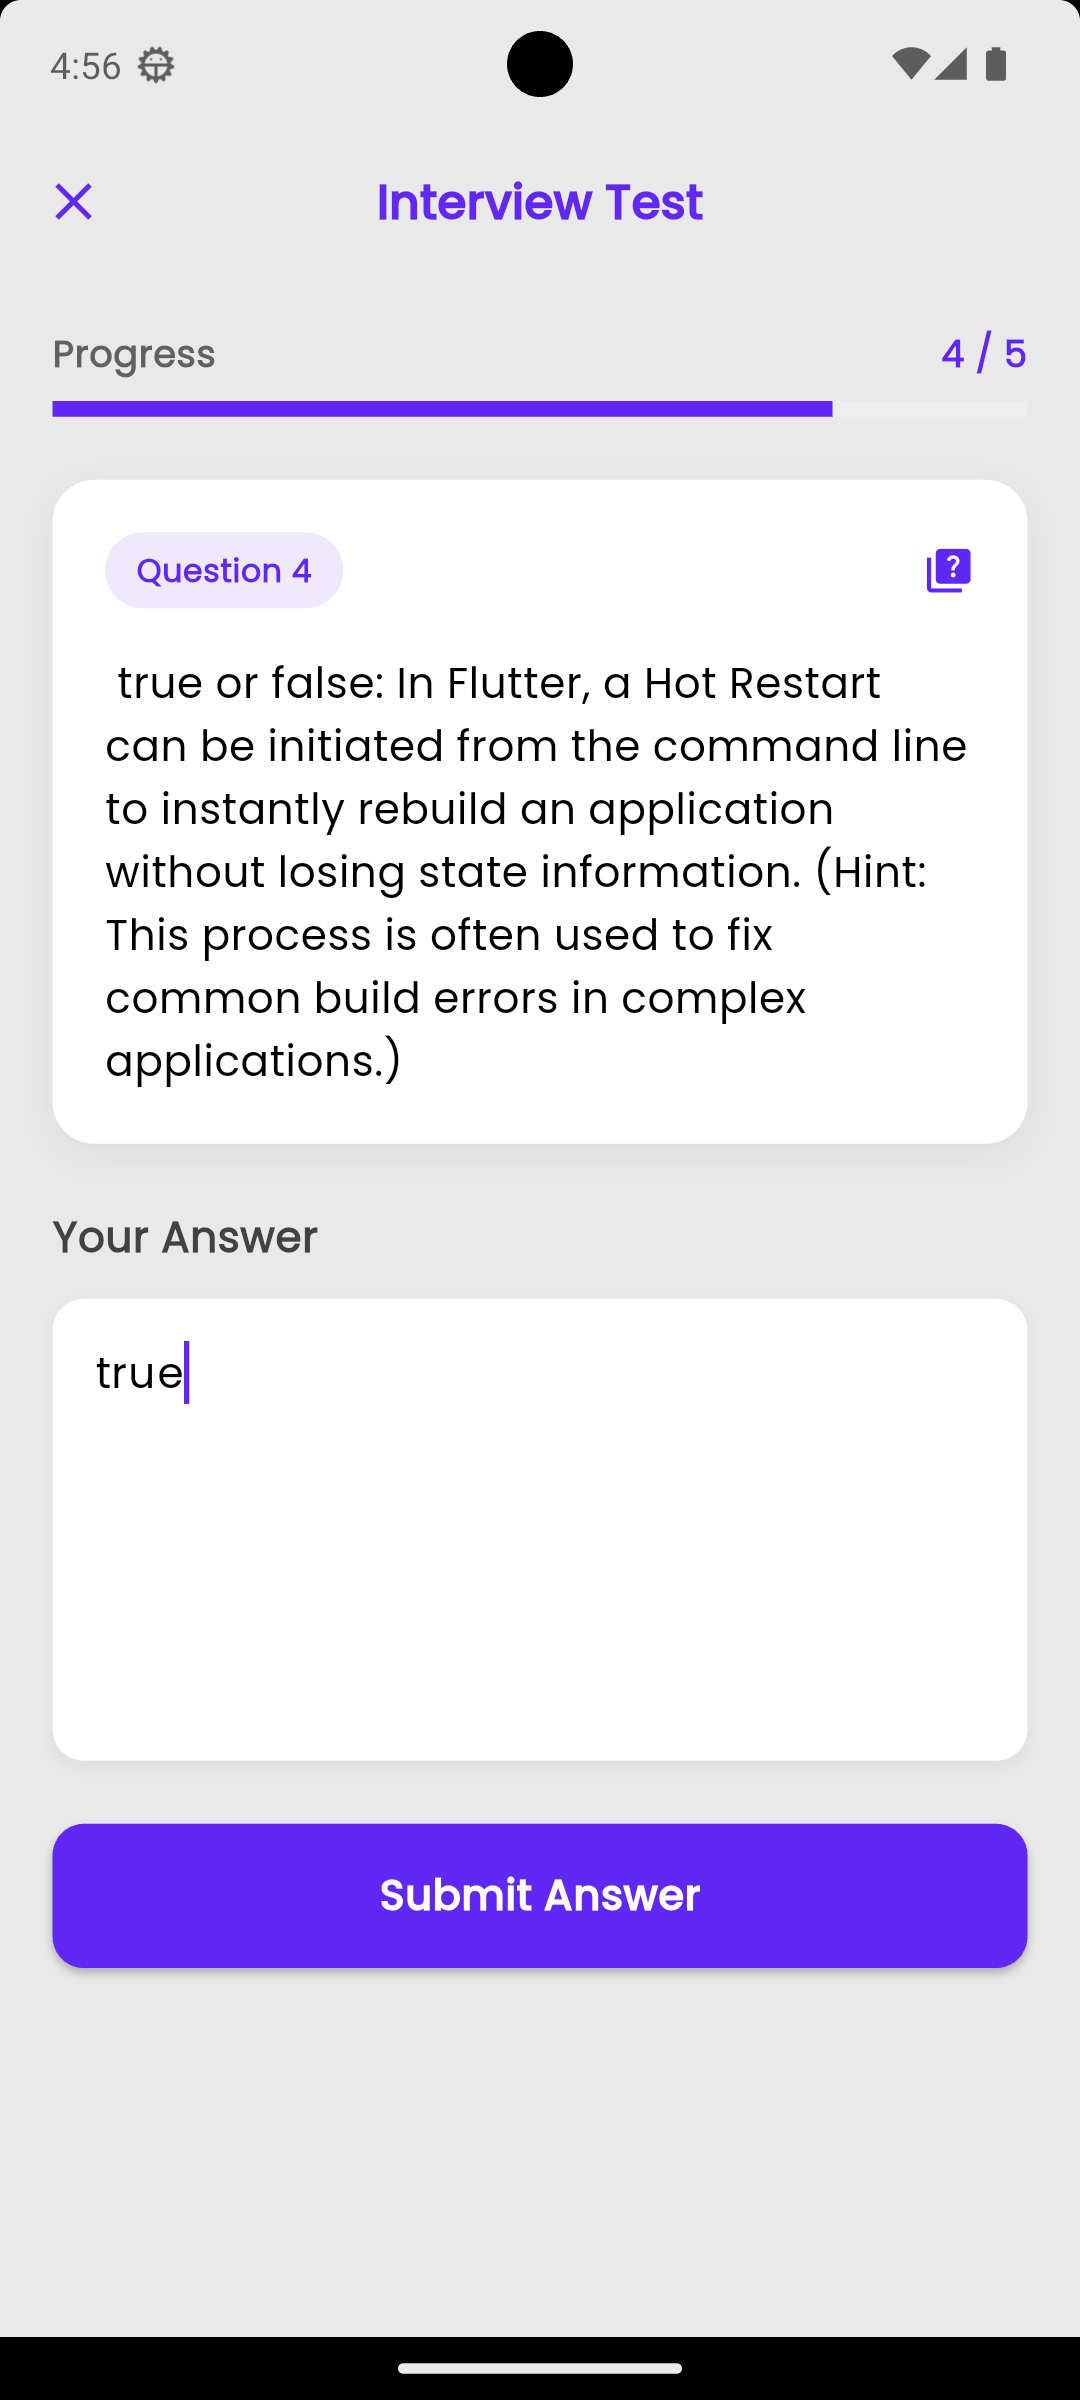
\includegraphics[height=0.45\textheight, keepaspectratio]{images/submitanswerInterview.png}
        \caption{Interface Mobile – Envoyer la réponse – étape 2}
    \end{minipage}

    \vspace{1em}

    % Bottom row: two more mobile screenshots side by side
    \begin{minipage}[b]{0.45\textwidth}
        \centering
        
\includegraphics[height=0.45\textheight, keepaspectratio]{images/EvaluationInterview.png}
        \caption{Interface Mobile – Résultat de l'évaluation de la réponse – étape 3}
    \end{minipage}
    \hfill
    \begin{minipage}[b]{0.45\textwidth}
        \centering
        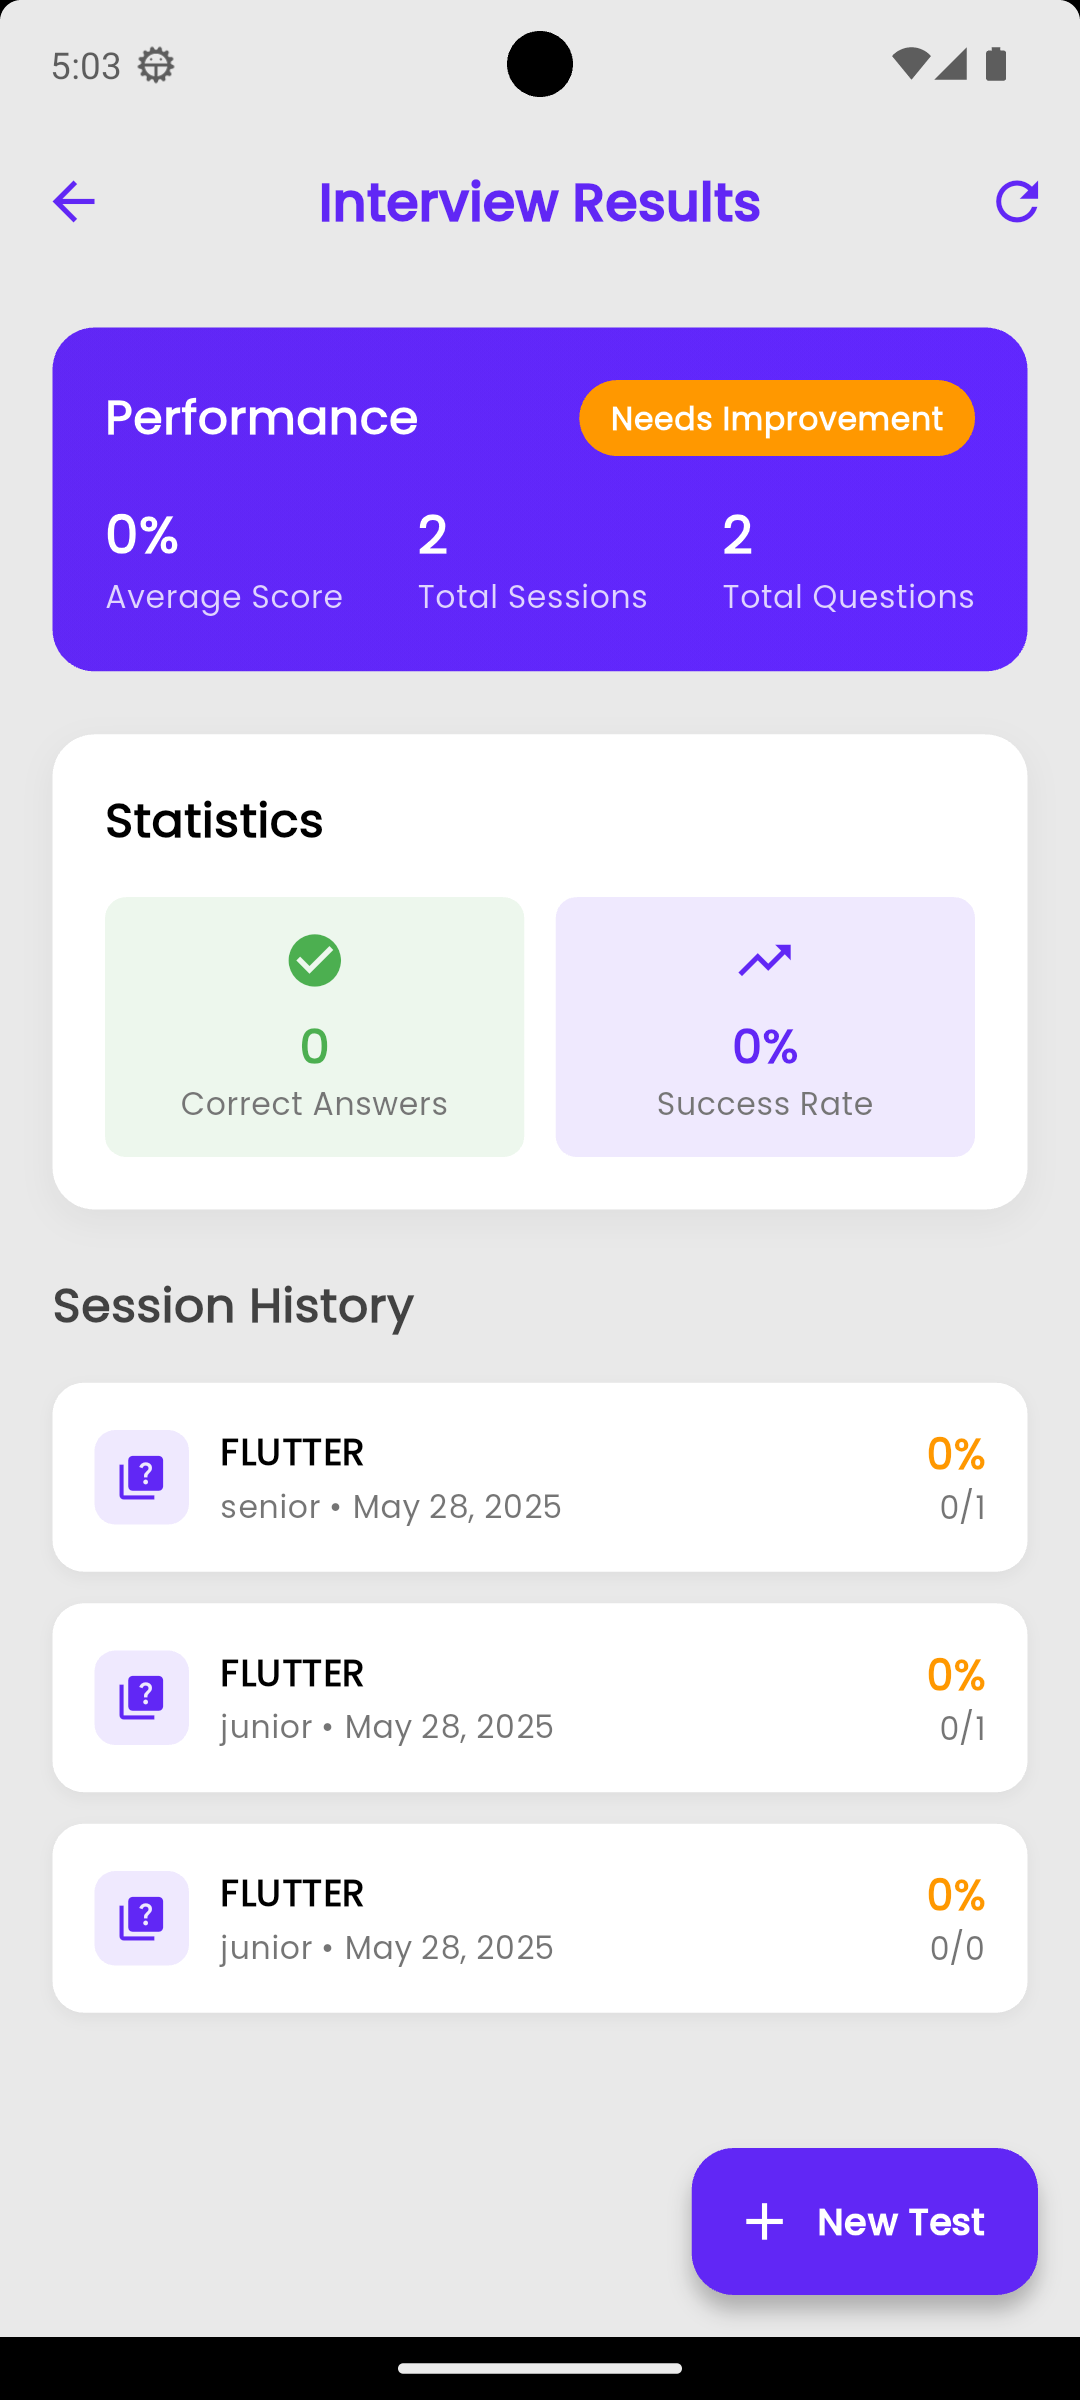
\includegraphics[height=0.45\textheight, keepaspectratio]{images/interviewresult.png}
        \caption{Interface Mobile – Voir le résultat et le score de l'Interview – étape 4}
    \end{minipage}

\end{figure}
\begin{figure}[H]
    \centering

    % Image 1
    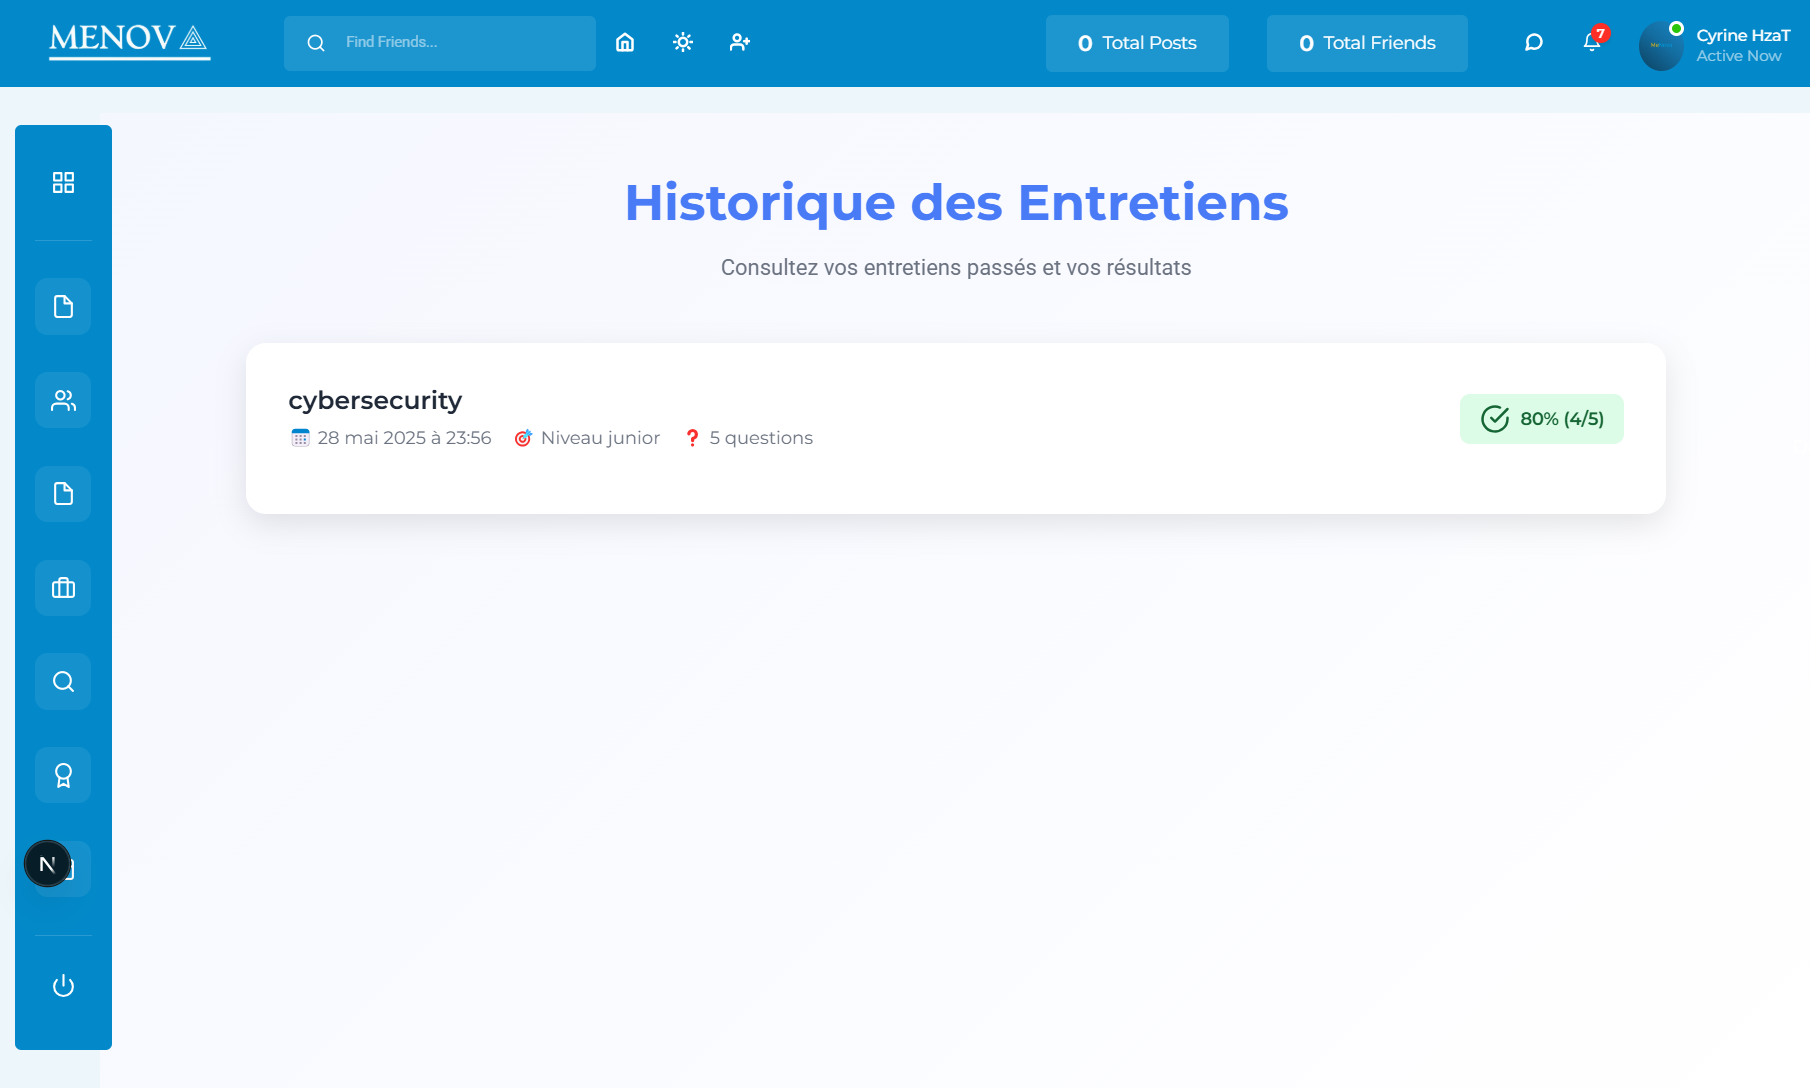
\includegraphics[width=0.9\textwidth, height=0.3\textheight, keepaspectratio]{images/interviewHistorique.png}
    \caption{Interface Web – Historiques des entretiens – étape 5}

   

    % Image 2
    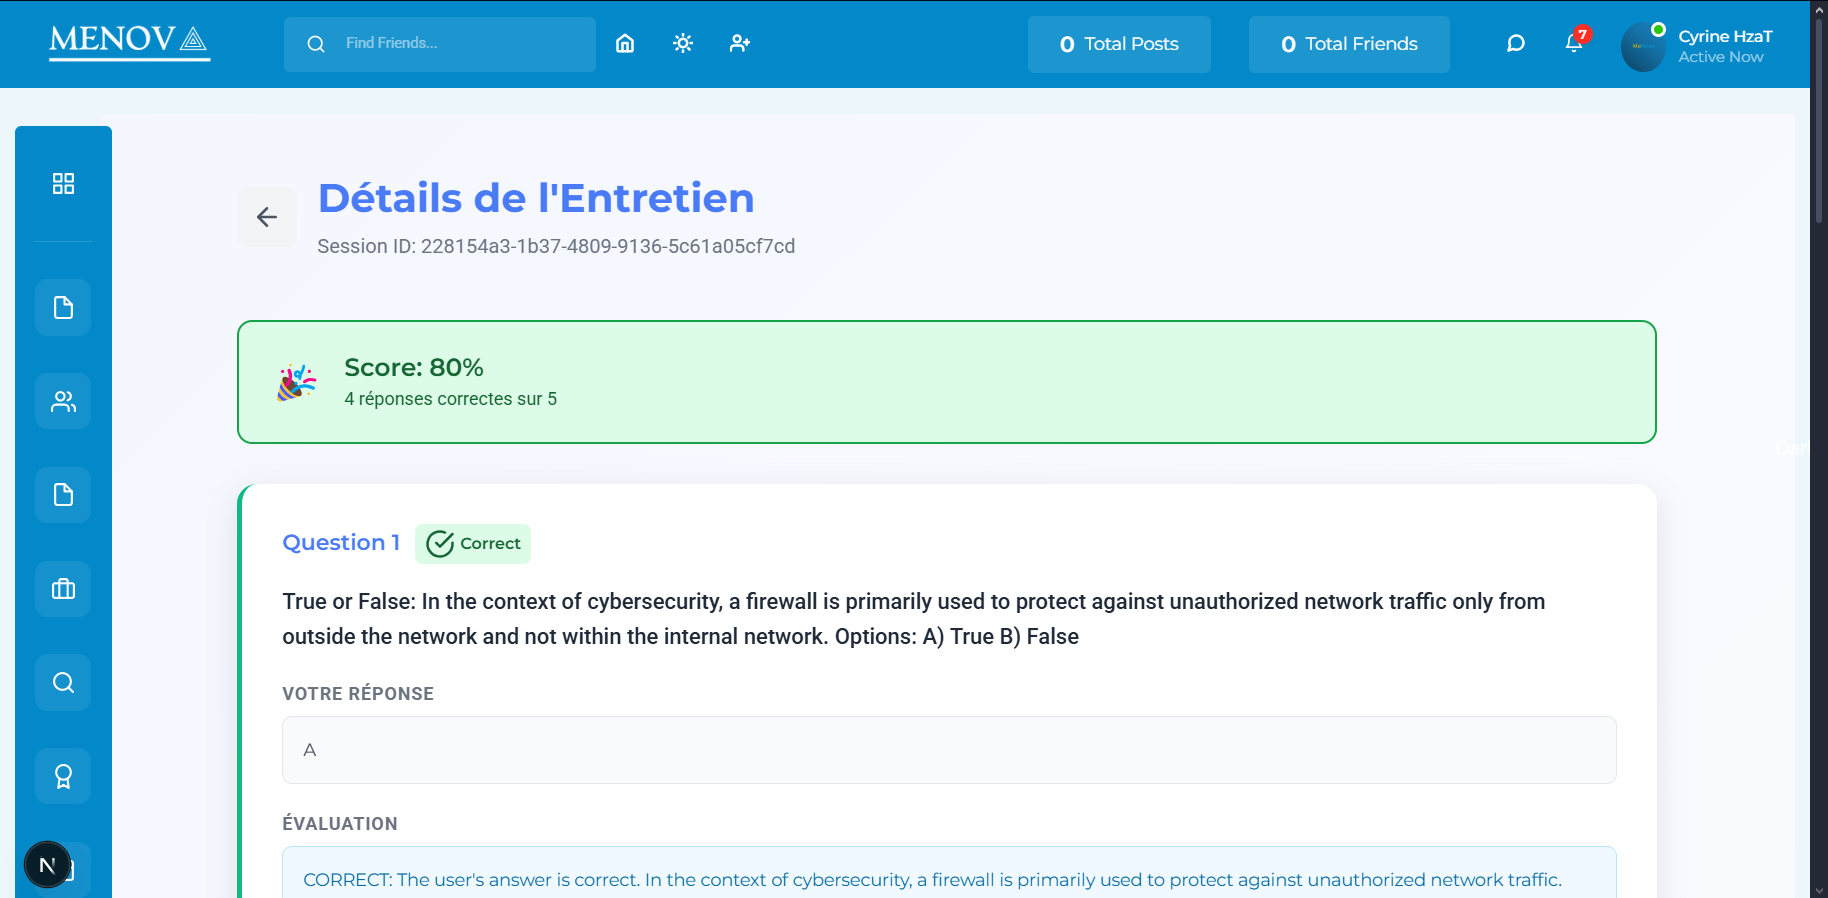
\includegraphics[width=0.9\textwidth, height=0.3\textheight, keepaspectratio]{images/interviewHistoriqueDetails.png}
    \caption{Interface Web – Voir détails d'un Historique – étape 6}

   

    % Image 3
    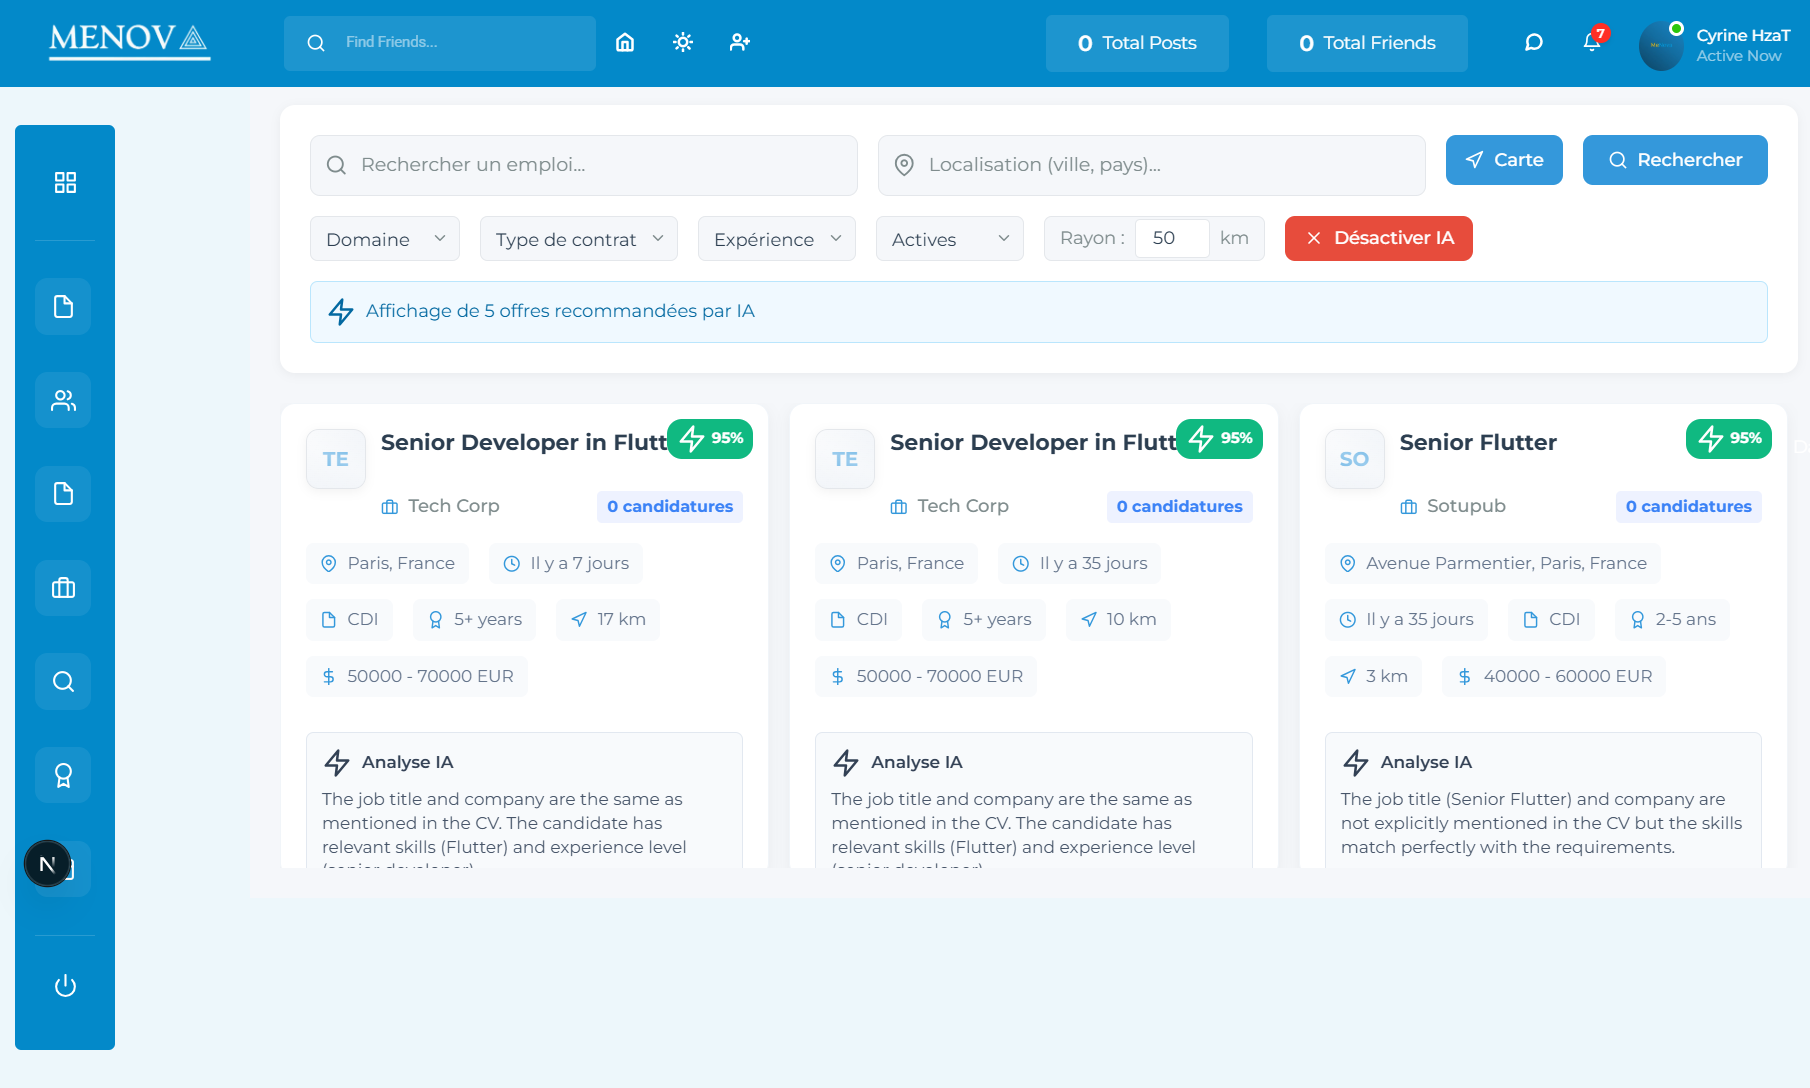
\includegraphics[width=0.9\textwidth, height=0.3\textheight, keepaspectratio]{images/matchingOffers.png}
    \caption{Interface Web – Match les Offres d'emploi – étape 1}


    \label{fig:web-interfaces-combined}
\end{figure}


\newpage
\section*{Conclusion}
\addcontentsline{toc}{section}{Conclusion}
Le Sprint 5 a permis d’enrichir la plateforme SafeTrack avec un microservice d’intelligence artificielle avancé, entièrement intégré à l’architecture existante. Ce microservice, exposé via l’API Gateway principale, assure une communication fluide avec les différents services du système tels que la localisation en temps réel, la gestion des alertes et les zones de sécurité, garantissant ainsi une expérience utilisateur cohérente et centralisée.
L’intégration d’un modèle de langage exécuté localement via Ollama, combiné à une architecture RAG, représente une étape importante dans l’évolution de SafeTrack vers un système intelligent et autonome. Cette approche permet non seulement de générer des analyses contextuelles précises, mais aussi de garantir la confidentialité des données sensibles en évitant le recours systématique à des services cloud externes.
L’utilisation du système RAG renforce considérablement la capacité de la plateforme à fournir des recommandations pertinentes et adaptées aux situations détectées. Grâce à l’exploitation d’une base de connaissances spécialisée en sécurité et en gestion des alertes, SafeTrack est désormais capable d’expliquer les événements, de proposer des actions immédiates et d’accompagner les parents et institutions dans la prise de décision.
Ce travail constitue une évolution majeure dans l’architecture du projet, en introduisant une couche d’intelligence qui améliore la détection des risques, la compréhension des alertes et la qualité des recommandations. Il ouvre également la voie à plusieurs améliorations futures, notamment l’enrichissement des modèles prédictifs, l’optimisation des performances en temps réel et le développement d’un assistant encore plus personnalisé pour le suivi et la protection des enfants.
